\documentclass{beamer}
%\usetheme{Warsaw}
\usepackage{color}
\usepackage{lmodern}
\usepackage[T1]{fontenc}
\usepackage[utf8x]{inputenc}
\usepackage[ngerman]{babel}
\usepackage{graphicx}
%\usepackage{inconsolata} % TT font
\usepackage{amsmath}
\usepackage{amsfonts}
\usepackage{textcomp}
\usepackage{hyperref}
\usepackage{url}
\usepackage{array}

\title{Suffix Arrays und BWT}
\author{Tobias Harrer}
\date{19.11.12}
 
\begin{document}
\maketitle
\frame{\tableofcontents[currentsection]}
 
\section{Suffix Arrays}
%%%%%
\subsection{Grundlagen}
\begin{frame} %%Eine Folie
  \frametitle{Suffix Arrays} %%Folientitel
  \begin{Definition} %%Definition
    Sei T ein String der Länge n über $\Sigma$ und $T_{i,j} (i\leq j)$ der Substring von i bis j, dann ist $T_{i,n}$ ein Suffix von T. Das Suffix Array von T ist die Permutation der Startindizes i der alphabetischen geordneten Suffixes $T_{i,n}$ von T.
  \end{Definition}
  Anmerkung: jeder String T endet mit \$ \newline
  $\forall c \in \Sigma : \$ < c$
\end{frame}
\begin{frame}
\frametitle{Suffix Arrays - Beispiel} %%Folientitel
T = \glqq abacabra\$\grqq\\[5mm]

\begin{tabular}{r|l<{\ttfamily} r<{\ttfamily}}
\textbf{i $T_{i,n}$} & \textbf{alphabetisch geordnet}\\\hline
1 & abacabra\$ & \$ 9\\
2 & bacabra\$ & a\$ 8\\
3 & acabra\$ & abacabra\$ 1\\
4 & cabra\$ & abra\$ 5\\
5 & abra\$ & acabra\$ 3\\
6 & bra\$ & bacabra\$ 2\\
7 & ra\$ & bra\$ 6\\
8 & a\$ & cabra\$ 4\\
9 & \$ & ra\$ 7\\
\end{tabular}\\[5mm]
Das Suffix Array von T lautet: \newline
{\ttfamily
\qquad 1 2 3 4 5 6 7 8 9 \textrightarrow\ \textbf{i}\newline
\qquad 9 8 1 5 3 2 6 4 7 \textrightarrow\ \textbf{S(i)}
}
\end{frame}
%%%%
\subsection{Suffix Arrays aus Suffix Trees}
\begin{frame}
\frametitle{Suffix Arrays aus Suffix Trees} %%Folientitel
\begin{itemize}
\item Sortierung durch z.B. mergeSort in $\mathcal{O}(n\cdot log (n))$
\item Ein Suffix Array kann aus des Blättern eines Suffix Trees durch Tiefensuche hergeleitet werden: T = \glqq abacabra\$\grqq\newline
\end{itemize}
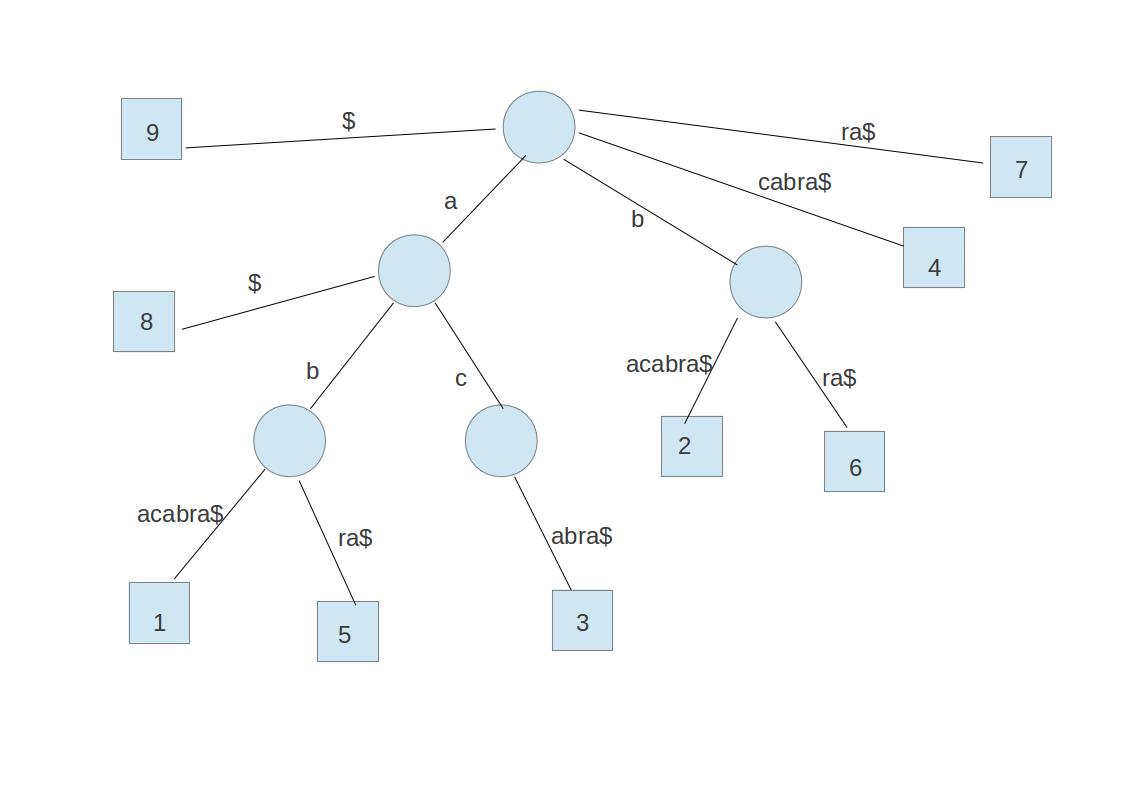
\includegraphics[height=0.5\textheight]{SuffixTree.jpg}
\end{frame}
%%%%
\subsection{Anwendung von Suffix Arrays}
\begin{frame}
\frametitle{Anwendung von Suffix Arrays}
\begin{itemize}
\item Finde Pattern p (\glqq cab\grqq) in String T (\glqq abacabra\grqq)
\item Naiver Ansatz: \glqq schiebe\grqq\ p über T: \newline
{\ttfamily
abacabra \newline
cab\textrightarrow \newline
...\newline
abacabra \newline
. . cab
}
\item Problem: $\mathcal{O}(n\cdot m)$
\end{itemize}
\end{frame}
%
\begin{frame}
\frametitle{Anwendung von Suffix Arrays}
\begin{itemize}
\item Vorteil: alle Suffixes lexikografisch sortiert
\item p \glqq cab\grqq ist Präfix $T_{1,i}$ des Suffix $T_{4,n}$: \newline
\begin{tabular}{r|l<{\ttfamily}}
\textbf{i} & \textbf{$T_{i,n}$}\\\hline
9 & \$\\
8 & a\$\\
1 & abacabra\$\\
5 & abra\$\\
3 & acabra\$\\
2 & bacabra\$\\
6 & bra\$\\
4 & {\color{red}\textbf{cab}}ra\$\\
7 & ra\$\\
\end{tabular}
\item Beste Suchstrategie in sortiertem Array?
\end{itemize}
\end{frame}
%
\begin{frame}
\frametitle{Anwendung von Suffix Arrays}
\begin{itemize}
\item Binäre Suche, Vergleich von \glqq cab\grqq mit $T{i,i+3}$:\newline
\begin{tabular}{l|l<{\ttfamily}}
\textbf{i} & $T_{i,n}$\\\hline
9 & \$\\
8 & a\$\\
1 & abacabra\$\\
5 & abra\$\\
3 & \color{red}\textbf{aca}\color{black}bra\$\ \glqq cab\grqq $>$ \glqq aca\grqq \textrightarrow zweite Hälfte\\
2 & bacabra\$\\
6 & bra\$\\
4 & cabra\$\\
7 & ra\$\\
\end{tabular}
\end{itemize}
\end{frame}
\begin{frame}
\frametitle{Anwendung von Suffix Arrays}
\begin{tabular}{r|l<{\ttfamily}}
\textbf{i} & $T_{i,n}$\\\hline
3 & acabra\$\\
2 & bacabra\$\\
6 & {\color{red}\textbf{bra}}\$ \glqq cab\grqq $>$ \glqq bra\grqq \textrightarrow zweite Hälfte\\
4 & cabra\$\\
7 & ra\$\\
\end{tabular}
\end{frame}
\begin{frame}
\frametitle{Anwendung von Suffix Arrays}
\begin{itemize}
\item
\begin{tabular}{r|l<{\ttfamily}}
\textbf{i} & $T_{i,n}$\\\hline
6 & bra\$\\
4 & {\color{red}\textbf{cab}}ra\$ \glqq cab\grqq  $=$ \glqq cab\grqq  \textrightarrow Pattern ist $T_{4,4+3}$\\
7 & ra\$\\
\end{tabular}\newline
\item Anschliessend Suche nach weiteren Vorkommen von p.
\item Suche in $\mathcal{O}(log (n))$
\end{itemize}
\end{frame}
\begin{frame}
\frametitle{Zusammenfassung: Binäre Suche in Suffix Arrays}
\begin{itemize}
\item Finden der n Suffixes in T: $\mathcal{O}(n)$
\item Alphabetisch Sortieren des Suffix Arrays: $\mathcal{O}(n\cdot log (n))$
\item Binäre Suche eines Patterns in T: $\mathcal{O}(log (n))$
\item Insgesamt $\mathcal{O}(n \cdot log (n))$ (oder $m \cdot log (n)$?)
\end{itemize}
\end{frame}
%%%%%
\subsection{Backward Search}
\begin{frame}
\frametitle{Backward Search}
\begin{itemize}
\item Grundlage: Suffix Array
\item Neu: keine binäre Suche, finden von zB \glqq b\grqq mit Array C[\glqq b\grqq ] = 5
\item Vorheriger Buchstabe $T_{A[i]-1}$ des Suffix $T_{A[i],n}$
\end{itemize}
\end{frame}

\begin{frame}
\frametitle{Bsp.: Suche von p = \glqq abra\grqq }
T = \glqq abacabra\$\grqq\\[5mm]
\begin{tabular}{l<{\ttfamily}|c<{\ttfamily} c<{\ttfamily}c<{\ttfamily} l<{\ttfamily}}
\textbf{i} & $A[i]$ & $T_{A[i]-1}$ & $T_{A[i],n}$\\\hline
1 & 9 & a & \$ \\
2 & 8 & r & a\$ \\
3 & 1 & \$ & abacabra\$ \\
4 & 5 & c & abra\$ \\
5 & 3 & b & acabra\$ \\
6 & 2 & a & bacabra\$ \\
7 & 6 & a & bra\$ \\
8 & 4 & a & cabra\$ \\
9 & 7 & b & ra\$ \\
\end{tabular}\\[5mm]
\begin{itemize}
\item \glqq abr{\color{red}\textbf{a}}\grqq von hinten: alle \texttt{a}, von C[\glqq a\grqq ]+1 bis C[\glqq b\grqq ]
\end{itemize}
\end{frame}
\begin{frame}
\frametitle{Bsp.: Suche von p = \glqq abra\grqq (Schritt 1)}
\begin{itemize}
\item Darunter alle \glqq a\grqq mit Vorgänger \glqq r\grqq\\[5mm]
\begin{tabular}{l<{\ttfamily}|c<{\ttfamily} c<{\ttfamily}c<{\ttfamily} l<{\ttfamily}}
i & $A[i]$ & $T_{A[i]-1}$ & $T_{A[i],n}$\\\hline
\textbf{2} & \textbf{8} & \color{red}\textbf{r} & \textbf{a\$} \\
3 & 1 & \$ & abacabra\$ \\
4 & 5 & c & abra\$ \\
5 & 3 & b & acabra\$ \\
\end{tabular}\\[5mm]
\item Weiter zu i = C[\glqq r\grqq]+1 = 9
\end{itemize}
\end{frame}
\begin{frame}
\frametitle{Bsp.: Suche von p = \glqq abra\grqq (Schritt 2)}
\begin{itemize}
\item Suche \glqq a\color{red}\textbf{b}\color{black}ra\grqq in r mit Vorgänger b
\begin{tabular}{l<{\ttfamily}|c<{\ttfamily} c<{\ttfamily}c<{\ttfamily} r<{\ttfamily}}
\textbf{i} & $A[i]$ & $T_{A[i]-1}$ & $T_{A[i],n}$\\\hline
. & . & . & .\\
5 & 3 & b & acabra\$ \\
. & . & . & .\\
\textbf{9} & \textbf{7} & \color{red}\textbf{b} & \textbf{ra\$} \\
\end{tabular}
\item b ist bei i = 5 bereits \textit{einmal} in $T_{A[i]-1}$ vorgekommen \textrightarrow suche von C[\glqq b\grqq]+1\textit{+1} bis C[\glqq c\grqq], d.h. bei i = 7
\end{itemize}
\end{frame}
\begin{frame}
\frametitle{Bsp.: Suche von p = \glqq abra\grqq (Schritt 3)}
\begin{itemize}
\item Finde alle \glqq{\color{red}\textbf{a}}bra\grqq  in b mit Vorgänger \glqq a\grqq:\\[5mm]
\begin{tabular}{l<{\ttfamily}|c<{\ttfamily} c<{\ttfamily}c<{\ttfamily} r<{\ttfamily}}
\textbf{i} & $A[i]$ & $T_{A[i]-1}$ & $T_{A[i],n}$\\\hline
1 & 9 & a & \$ \\
. & . & . & .\\
6 & 2 & a & bacabra\$ \\
\textbf{7} & \textbf{6}  & \color{red}\textbf{a} & \textbf{bra\$} \\
\end{tabular}\\[5mm]
\item Da bei i = 1 und 6 a bereits \textit{zweimal} in $T_{A[i]-1}$ vorkam \textrightarrow suche von C[\glqq a\grqq]+1\textit{+2} bis C[\glqq b\grqq], d.h. bei i = 4
\end{itemize}
\end{frame}
\begin{frame}
\frametitle{Bsp.: Suche von p = \glqq abra\grqq  (Schritt 4)}
\begin{tabular}{l<{\ttfamily}|c<{\ttfamily} c<{\ttfamily}c<{\ttfamily} r<{\ttfamily}}
\textbf{i} & $A[i]$ & $T_{A[i]-1}$ & $T_{A[i],n}$\\\hline
4 & 5 & c & \color{red}\textbf{abra\$} \\
\end{tabular}\\[5mm]
\begin{itemize}
\item Nach 4 Schritten (= Länge m von p) ist das Pattern gefunden $\rightarrow \mathcal{O}(m)$
\item Problem: z.B. \textit{wie oft ist \glqq b\grqq  in Spalte $T_{A[i]-1}$ vor i = 5} erfordert lineares Durchsuchen von $T_{A[i]-1}\ \rightarrow\ \mathcal{O}(m\cdot n)$.
\item Effizientes Vorgehen nötig, sonst Laufzeit wie bei naiver Suche!
\end{itemize}
\end{frame}
\begin{frame}
\frametitle{Lösung: Funktion Occ(c,i)}
\begin{itemize}
\item Die Spalte des Vorgänger-Buchstaben $T_{A[i]-1}$ nennen wir ab jetzt $L_{1,n}$
\item Für alle c aus $\Sigma$ sei $B^{c}$ ein Bit-Vektor mit $B^{c}[i] = 1$ falls $L_{i} = c$
\item Eine weitere Funktion $rank_{b}(B,i)$ liefert die Anzahl von zB b=1 in B vor i, s.d $rank_{1}(B^{c},i) = Occ(c,i)$.
\item Dies benötigt linear mehr Speicher, doch der Zugriff durch rank ist konstant, s.d. $\mathcal{O}(m)$ insgesamt garantiert ist.
\item Wavelet Trees?
\end{itemize}
\end{frame}
\begin{frame}
\subsection{Forward Searching}
\frametitle{Forward Searching}
\begin{itemize}
\item Vorherige Position: $LF(i) = C[L_i] + Occ(L_i,i)$
\item Während beim Backward Searching ein Suffix auf das vorhergehende abgebildet wird, ist es hier umgekehrt
\item Inverse Funktion $\Psi(i) = i'$, s.d. A[i'] = (A[i] mod n)+1 bildet die Pos. eines Suffix auf die seines Nachfolgers ab
\end{itemize}
\end{frame}
\begin{frame}
\frametitle{Bsp.: $\Psi$ zu T = \glqq abacabra\$\grqq}
\begin{tabular}{l<{\ttfamily}|c<{\ttfamily} c<{\ttfamily}c<{\ttfamily} c<{\ttfamily}c<{\ttfamily}c<{\ttfamily} r<{\ttfamily}}
i & $A[i]$ & $\Psi$ & newF & $T_{A[i],n}$ \\\hline
1 & 9 & 3 & 1 &\$\\
2 & 8 & 1 & 1 &a\$\\
3 & 1 & 6 & 0 &abacabra\$\\
4 & 5 & 7 & 0 &abra\$\\
5 & 3 & 8 & 0 &acabra\$\\
6 & 2 & 5 & 1 &bacabra\$\\
7 & 6 & 9 & 0 &bra\$\\
8 & 4 & 4 & 1 &cabra\$\\
9 & 7 & 2 & 1 &ra\$\\
\end{tabular}
\end{frame}
\begin{frame}
\frametitle{Suche von p in T}
\begin{itemize}
\item Falls $\forall c: c \in \Sigma \Rightarrow c \in T$ ex. $\sigma$ aufsteigende Zahlenfolgen in $\Psi$: 3; 1,6,7,8; 5,9; 4; 2;
\item Diese zeigen an, wo sich der erste Buchstabe des Suffix ändert. Als Bitvektor newF = 110001011
\item Die Suche von p erfolgt binär, wobei p ein Prefix des jew. Suffix ist, welches durch rekursives Folgen von $\Psi(i)$ \textit{ohne das Suffix Array} gefunden werden kann
\item Der jew. erste Buchstabe $T_{A[i]}$ des Suffixes $T_{A[i],n}$ wird durch $rank(newF,i)$ ermittelt. Falls zB $rank(newF,i) = 2$ ist c = \glqq a\grqq.
\end{itemize}
\end{frame}
\begin{frame}
\frametitle{Fazit Forward Searching}
\begin{itemize}
\item $\Psi$ ersetzt A[i].
\item Weder A[i] noch T sind zur Suche von p in T nötig
\item $\Psi$ kann durch \textit{gap-encoding} weiter komprimiert werden.
\end{itemize}
\end{frame}
\section{Burrows-Wheeler Transformation}
\begin{frame}
\frametitle{Burrows-Wheeler Transformation}
\begin{itemize}
\item Die BWT ist eine Permutation von T, s.d. an jeder Stelle des Suffix Arrays der vorherige Buchstabe angehängt wird:
\end{itemize}
\begin{Definition}
Sei $T_{1,n}$ ein String und A[1,n] sein Suffix Array. Dann ist die BWT $T_{1,n}^{bwt}$ von T: \newline $T_{i}^{bwt} = T_{A[i]-1}$ $\forall 1 \leq i \leq n$ ausser A[i] = 1 $\Rightarrow$ $T_{i}^{bwt} = T_n = \$ $
\end{Definition}
\end{frame}
\begin{frame}
\frametitle{Anschauliches Beispiel, T = \glqq abacabra\$\grqq}
\begin{tabular}{l<{\ttfamily} c<{\ttfamily} r<{\ttfamily}}
\textbf{Permutationen} & \textbf{alph. geordnet} & $F\ldots L = T^{bwt}$ \\\hline
abacabra\$ & \$abacabra & \$...a \\
bacabra\$a & a\$abacabr & a...r \\
acabra\$ab & abacabra\$ & a...\$ \\
cabra\$aba & abra\$abac & a...c \\
abra\$abac & acabra\$ab & a...b \\
bra\$abaca & bacabra\$a & b...a \\
ra\$abacab & bra\$abaca & b...a \\
a\$abacabr & cabra\$aba & c...a \\
\$abacabra & ra\$abacab & r...b \\
\end{tabular}\\[5mm]
\begin{itemize}
\item $T^{bwt}$ = ar\$cbaaab
\item BWT Permutation besser für weitere Komprimierung von T als T selbst
\end{itemize}
\end{frame}
\begin{frame}
\frametitle{BWT Rücktransformation}
\begin{itemize}
\item Da $L_i$ $F_i$ voransteht, kann T aus $T^{bwt}$ wie folgt wiederhergestellt werden:
\end{itemize}
\begin{tabular}{l<{\ttfamily} c<{\ttfamily} c<{\ttfamily}c<{\ttfamily} r<{\ttfamily}}
F...L & nach links &sortiert& L links angehängt\\\hline
\$...a &...a\$ &...\$a&...a\$a\\
a...r &...ra &...a\$&...ra\$\\
a...\$ &...\$a &...ab&...\$ab\\
a...c &...ca &...ab&...cab\\
a...b &...ba &...ac&...bac\\
b...a &...ab &...ba&...aba\\
b...a &...ab &...br&...abr\\
c...a &...ac &...ca&...aca\\
r...b &...br &...ra&...bra\\
\end{tabular}
\begin{itemize}
\item Reihe L = $T^{bwt}$ bekannt, F wird aus L alph. sortiert
\item Verschieben \glqq nach links\grqq, sortieren
\item L = $T^{bwt}$ links \glqq anhängen, sortieren...
\end{itemize}
\end{frame}
\begin{frame}
\frametitle{BWT Rücktransformation}
Nach n Durchgängen ist die Matrix wiederhergestellt:\\[5mm]
\begin{tabular}{l<{\ttfamily}}
\$abacabra \\
a\$abacabr \\
\color{red}\textit{abacabra}\$ \\
abra\$abac \\
acabra\$ab \\
bacabra\$a \\
bra\$abaca \\
cabra\$aba \\
ra\$abacab \\
\end{tabular}\\[5mm]
T ist derjenige String, der mit \glqq\$\grqq endet.
\end{frame}
% Zusammenfassung
\begin{frame}
 \frametitle{Zusammenfassung}
\end{frame}

\end{document}